\documentclass[tikz,border=3pt]{standalone}
\usepackage[utf8]{inputenc}
\usepackage[T1]{fontenc}
\usepackage{lmodern}
\renewcommand{\familydefault}{\sfdefault}
\usepackage{sansmath}\sansmath
\usepackage{chemfig}
\usepackage{pgfplots}\pgfplotsset{compat=1.18,/pgf/number format/use comma,/pgf/number format/1000 sep={.}}
\usetikzlibrary{arrows.meta,calc,positioning,decorations.pathmorphing,patterns}
% paleta del sitio
\definecolor{nar}{HTML}{E8680C}\definecolor{narc}{HTML}{FFB35C}\definecolor{hielo}{HTML}{FFF3E8}
\definecolor{tinta}{HTML}{1D1D1F}\definecolor{gris}{HTML}{6E6E73}\definecolor{lila}{HTML}{7C5CF0}
\definecolor{azul}{HTML}{2F6FD6}\definecolor{menta}{HTML}{17A673}\definecolor{coral}{HTML}{E8342A}
\setchemfig{atom sep=2em,bond style={line width=0.8pt}}
\tikzset{lab/.style={font=\small\bfseries,text=nar},pie/.style={font=\footnotesize,text=tinta,align=center}}
\begin{document}
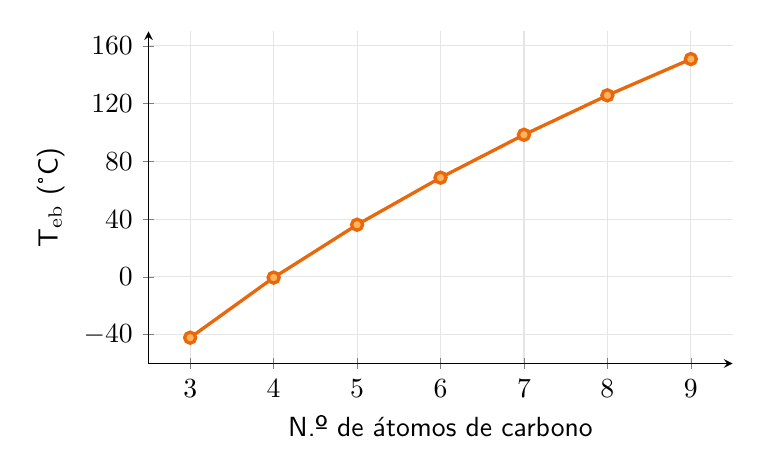
\begin{tikzpicture}
\begin{axis}[width=9cm,height=5.8cm,xlabel={N.º de átomos de carbono},ylabel={T$_\mathrm{eb}$ (°C)},axis lines=left,grid=major,grid style={gray!20},xmin=2.5,xmax=9.5,ymin=-60,ymax=170,xtick={3,...,9},ytick={-40,0,40,80,120,160}]
\addplot[nar,very thick,mark=*,mark options={fill=narc}] coordinates {(3,-42.1)(4,-0.5)(5,36.1)(6,68.7)(7,98.4)(8,125.7)(9,150.8)};
\end{axis}
\end{tikzpicture}
\end{document}
